\documentclass{beamer}
\usepackage[french]{babel}
\usepackage[utf8]{inputenc} % Set input encoding to Unicode UTF-8
\usepackage[T1]{fontenc} % Set character encoding to T1/Cork
\usepackage{minted}
\usepackage{svg}
\usepackage{hyphenat}
\usepackage{amssymb}
\usepackage{tabularx}
\usepackage{booktabs}
\usepackage{adjustbox}
\usepackage{csquotes}
\usepackage{float}

\newcommand\att[1]{\textnhtt{#1}}

\title{Projet de Bases de Données}
\author{Pradana \textbf{Aumars}
  \and
  David \textbf{Behrens}
  \and
  El Hadji Abdoul Aziz \textbf{Kane}
  \and
  Mohamed Lemine \textbf{Mohamed Ahmed}
  \and
  Mohamedou \textbf{Chrif M'hamed}}

\begin{document}
\frame{\titlepage}
\begin{frame}{Sommaire}
  \begin{enumerate}
  \item Analyse du problème
  \item Conception
  \item Schéma relationnel
  \item Analyse des fonctionnalités
  \item Bilan du projet
  \item Mode d'emploi du démonstrateur
  \end{enumerate}
\end{frame}
\begin{frame}{Analyse du problème: l'exemple de \att{Refuge}}
  
  \textbf{Propriétés}: 
\att{emailRef}, % email du refuge
\att{nomRef}, % nom du refuge
\att{numTel}, % numéro de téléphone (optionnel) du refuge
\att{secGeo}, % secteur géographique du refuge
\att{dateOuv}, % date d'ouverture du refuge
\att{dateFerm}, % date de fermeture du refuge
\att{nbrPlacesRepas}, % nombre de places pour les repas dans un refuge
\att{nbrPlacesDormir}, % nombre de places pour dormir dans un refuge
\att{textePrez}, % texte de présentation d'un refuge
\att{typePayement}, % type de paiement pour un refuge
\att{prixNuite} % prix d'une nuite dans un refuge

\textbf{Dépendances fonctionnelles}:
\att{emailRef}
$\rightarrow$
\att{nomRef},
\att{numTel},
\att{secGeo},
\att{dateOuv},
\att{dateFerm},
\att{nbrPlacesRepas},
\att{nbrPlacesDormir},
\att{textePrez},
\att{typePayement},
\att{prixNuite}

\textbf{Contraintes de valeur}:
$\att{dateOuv} < \att{dateFerm}$

$\att{nbrPlacesRepas} \geq 0$

$\att{nbrPlacesDormir} \geq 0$

$\att{typePayement} \in \{ \texttt{"espèce"}, \texttt{"chèque"}, \texttt{"carte-bleue"} \}$

$\att{prixNuite} \geq 0$
\end{frame}

\begin{frame}{Conception}
  \begin{figure}[H]
\includesvg[inkscapelatex=false, width=\textwidth]{schema}
\caption{Diagramme entité-association}
\end{figure}
\end{frame}

\begin{frame}{Schéma relationnel: les exemples de \att{Refuge} et \att{ReservationRefuge}}
\att{REFUGE}(\att{\underline{emailRef}}, \att{nomRef}, \att{numTel}, \att{secGeo}, \att{dateOuv}, \att{dateFerm}, \att{nbrPlacesRepas}, \att{nbrPlacesDormir}, \att{textePrez}, \att{typePayement}, \att{prixNuite})
\begin{itemize}
\item \textbf{Forme normale}: Non normalisé (\att{numTel} pourrait être \att{NULL})
\end{itemize}

\att{RESERVATION\_REFUGE}(\att{\underline{idReservRef}}, \att{dateReservRef}, \att{heureReservRef}, \att{nbrNuitsReserv}, \att{nbrRepasReserv}, \att{prixTotalReserv}, \att{emailRef}, \att{idUser})
\begin{itemize}
\item \textbf{Forme normale}: 3FNBCK
\item \att{emailRef} référence \att{REFUGE}(\att{emailRef})
\item \att{idUser} référence \att{COMPTE\_UTILISATEUR}(\att{idUser})
\end{itemize}
\end{frame}

\begin{frame}[fragile]{Implémentation de \att{Refuge}}
  \begin{minted}[fontsize=\scriptsize]{SQL}
    CREATE TABLE REFUGE (
    EMAIL VARCHAR(50) PRIMARY KEY,
    NOM VARCHAR(50),
    NUMTEL INT,
    SECGEO VARCHAR(50),
    DATEOUV DATE,
    DATEFERME DATE,
    CHECK (DATEOUV < DATEFERME),
    NBrREPAS INT,
    CHECK (NBrREPAS >= 0),
    NBrDORMIR INT,
    CHECK (NBrDORMIR >=0),
    TEXTE VARCHAR(50),
    TYPePAYEMENT VARCHAR(20),
    CHECK (TYPePAYEMENT IN ('espèces','chèque', 'carte-bleue')),
    PRIxNUITE DECIMAL,
    CHECK ( PRIxNUITE >= 0),
    PRIX DECIMAL
    );
  \end{minted}
\end{frame}

\begin{frame}{Bilan du projet}
  \begin{itemize}
  \item Toutes les fonctionnalités ont été implémentées.
  \item Départ un peu rapide, mais nous avons, par la suite, adopté une approche plus méthodique.
  \item Interface utilisateur suffisante mais à perfectionner au niveau de la gestion des exceptions et valeurs inattendues
  \end{itemize}
\end{frame}

\begin{frame}{Mode d'emploi du démonstrateur}
  \begin{columns}
    \begin{column}{0.7\textwidth}
        \begin{figure}[H]
      \includegraphics[width=\textwidth]{régles_utilisation.png}
\caption{Les règles d'utilisation}
\end{figure}
      \end{column}
    \begin{column}{0.3\textwidth}
        \begin{figure}[H]
      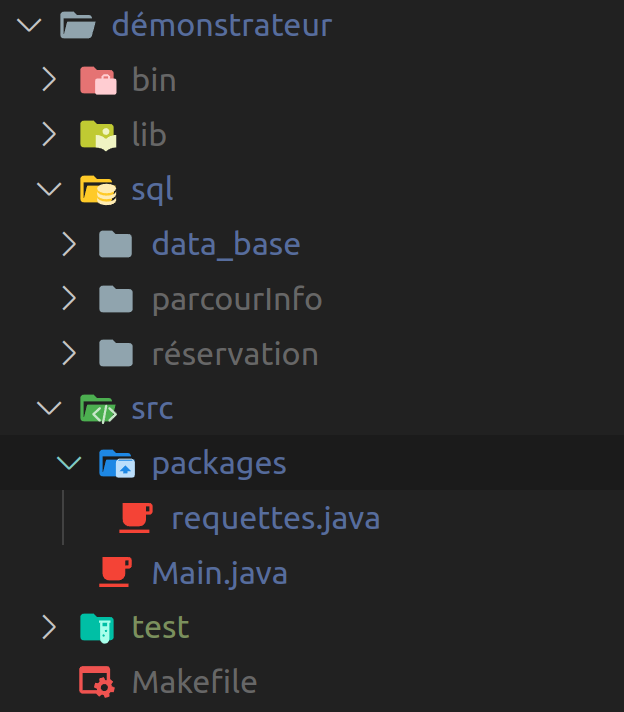
\includegraphics[width=\textwidth]{h_p.png}
\caption{La hiérarchie des fichiers}
\end{figure}
      \end{column}
    \end{columns}
  \end{frame}

  \begin{frame}{Mode d'emploi du démonstrateur}
        \begin{figure}[H]
      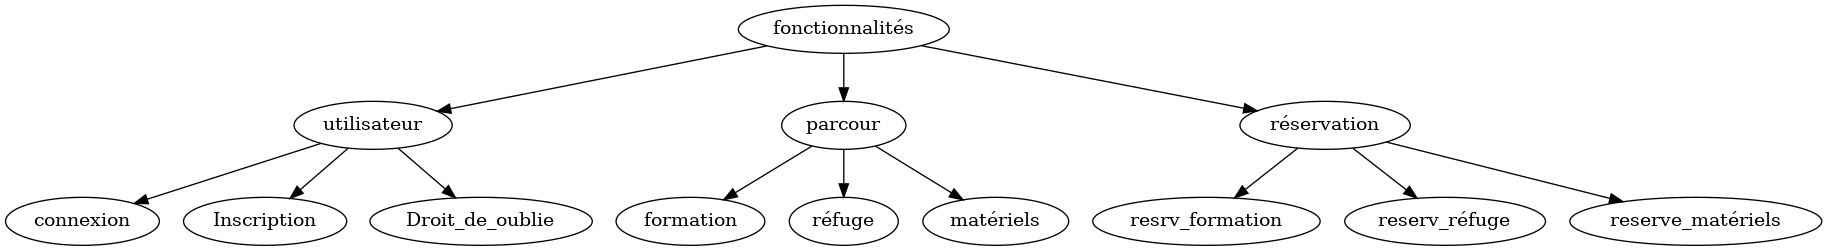
\includegraphics[width=\textwidth]{g.png}
\caption{L'organisation des fonctionnalités}
\end{figure}
  \end{frame}
\end{document}

% Local Variables:
% TeX-command-extra-options: "-shell-escape"
% End:
